\documentclass{sig-alternate}
\usepackage{graphicx}
\graphicspath{{./figures/}}

\begin{document}
%
% --- Author Metadata here ---
%\conferenceinfo{WOODSTOCK}{'97 El Paso, Texas USA}
\CopyrightYear{2014} % Allows default copyright year (20XX) to be over-ridden - IF NEED BE.
%\crdata{0-12345-67-8/90/01}  % Allows default copyright data (0-89791-88-6/97/05) to be over-ridden - IF NEED BE.
% --- End of Author Metadata ---

\title{Improving Hashtag Comprehension with Search and Text Summarization
%  \titlenote{(Produces the permission block, and copyright information). For use with SIG-ALTERNATE.CLS. Supported by ACM.}
}

\numberofauthors{3}
\author{
% 1st. author
\alignauthor
John Lanchantin\\
       \affaddr{University of Virginia}\\
       \affaddr{85 Engineer's Way}\\
       \affaddr{Charlottesville, VA 22904-4740}\\
       \email{jjl5sw@virginia.edu}
% 2nd. author
\alignauthor
Nicholas Janus\\
       \affaddr{University of Virginia}\\
       \affaddr{85 Engineer's Way}\\
       \affaddr{Charlottesville, VA 22904-4740}\\
       \email{ncj2ey@virginia.edu}
% 3rd. author
\alignauthor 
Weilin Xu\\
       \affaddr{University of Virginia}\\
       \affaddr{85 Engineer's Way}\\
       \affaddr{Charlottesville, VA 22904-4740}\\
       \email{xuweilin@virginia.edu}
}

\maketitle
\begin{abstract}
Posts on micro-blogging sites are often very hard to understand due to their informality. Hashtags represent one solution to this problem by acting as subject markers for posts. However, hashtags are often difficult to understand without reading through multiple posts or conversations. We attempt to solve hashtag comprehension problem by automatically understanding what hashtags mean, and displaying relevant documents or text from within those documents.
\end{abstract}

% A category with the (minimum) three required fields
\category{Information systems}{Information Retrieval}{Specialized Information Retrieval}
\keywords{Micro-blogging, Hashtag retrieval, hashtag prediction, hashtag comprehension}

\section{Introduction}
The Internet today, especially social network services such as twitter and Facebook, is filled with 'hashtags'. Hashtags are single tokens that use the character '\#' in front of the words, and are often composed of natural language n-grams abbreviations, or acronyms. The problem is that there is no structure to hashtags beyond the format of the '\#' character and no spaces, thus making it terribly difficult to understand them. Users often create hashtags that are slang, concatenations of many words, acronyms, or simply made up words.  \\
This problem's importance is highlighted by the type of information need that twitter itself satisfies.  \cite{twitternews} suggests that Twitter's primary function has less to do with social interaction and more to do with providing news.  The authors show that there is relaively little interaction via twitter's follower mechanism, which would suggest social interaction, but messages tend to propogate deeper into twitter's social network and persist for longer periods of time, supporting the assertion that it functions as more of a news network.  If twitter is a news and social network, then hashtags are equivalent to article titles.  If we don't understand the titles/hashtags, then how can we understand the articles/tweets?
There are certain hashtags that are very obvious to understand. For example, \#baseball, \#android, \#christmas each give a very clear cut definition of what they are about. On the other hand, there are many hashtags that are difficult to understand. For example. \#NCTL14, \#twitterblades, \#icymi, \#Saban14, are very difficult to understand because they are not real words and there is no hint of what they mean directly from the hashtag. Often times when directly searching these ambiguous hashtags on a search engine, the search engine does not return relevant results due to the fact that hashtags are so transient and there is no clear-cut definition.\\
An important task is to be able to automatically understand the underlying meaning behind a trending topic on social media. By understanding the meaning behind hashtags, we can further analyze what people are talking about. Often times, it does not become clear what someone is talking about until the meaning of his/her hashtag is understood, and it is frequently difficult to understand the hashtag due to their informality.\\
In order to understand the meaning behind hashtags, we propose a system that is able to return relevant documents for trending topics. Our solution consists of extracting tweets that use an inquired hashtag, and selecting proper keywords for query terms that can be searched using Bing.com. Related work is shown in section~\ref{sec:relatedWork}, we explain our proposed solution for hashtag understanding in  section~\ref{sec:implementation}, we explain our evaluation methodology and results in section~\ref{sec:evaluation}, and finally our conclusion and further work is shown in section~\ref{sec:conclusions}.
\\

\section{Related Work}
\label{sec:relatedWork}
The research surrounding hashtags covers a variety of topics including hashtag retrieval\cite{efron:retrieval}, hashtag prediction\cite{khabiri:predict}\cite{tagspace} for social media posts, or sentiment analysis for either the hashtag itself or the contents of the enclosing post.  Although these systems rely on an implicit understanding of the hash tag's meaning, they do not attempt to export such semantics.  Attempts to deliver the meaning of hashtags rely on crowdsourcing or manual annotation.\\
Currently, Twitter itself manually expands certain acronym hashtags (e.g. \#oitnb translates to ''orange is the new black"), but it does not explain what they mean. In addition, there are a few websites (e.g. tagdef.com) which attempt to explain hashtags by crowdsourcing definitions, but there is often no clear cut definition, and many definitions are highly opinionated. Both of the aforementioned methods do a poor job at explaining trending, or newly defined hashtags because they rely on the meaning of a hashtag over a long period of time, or have to wait until users explain the hashtag. In addition, the content quality is not as good as webpage links that give a more clearly defined explanation.
Our approach will have a much greater coverage of hashtag understanding and will not rely on manual annotation for an interpretation of the tag's meaning.  By giving access to our system via a browser plugin, our service will also be much more accessible and available to users of micro-blogging platforms.\\

\section{Approach and Implementation}
\label{sec:implementation}
The main idea of our approach is as follows. Based on all tweets that use the inquired hashtag, we create a query for a current search engine (Bing.com), and display relevant web pages and a short summary based on those web pages to the user. \\
The system flow works in the following way: the user issues a hashtag to find its meaning using a browser plugin, the system extracts and filters all tweets using that hashtag, generates a query based on the tweets, searches that query using bing, returns the links of the most relevant web pages, and generates a summarization of the text from the top web page. The links and summary are displayed to the user via the plugin. This is shown in figure \ref{fig:SystemArchitechture}. Each module is explained is explained in further detail in the following subsections.

\begin{figure}[h!]
     \fbox{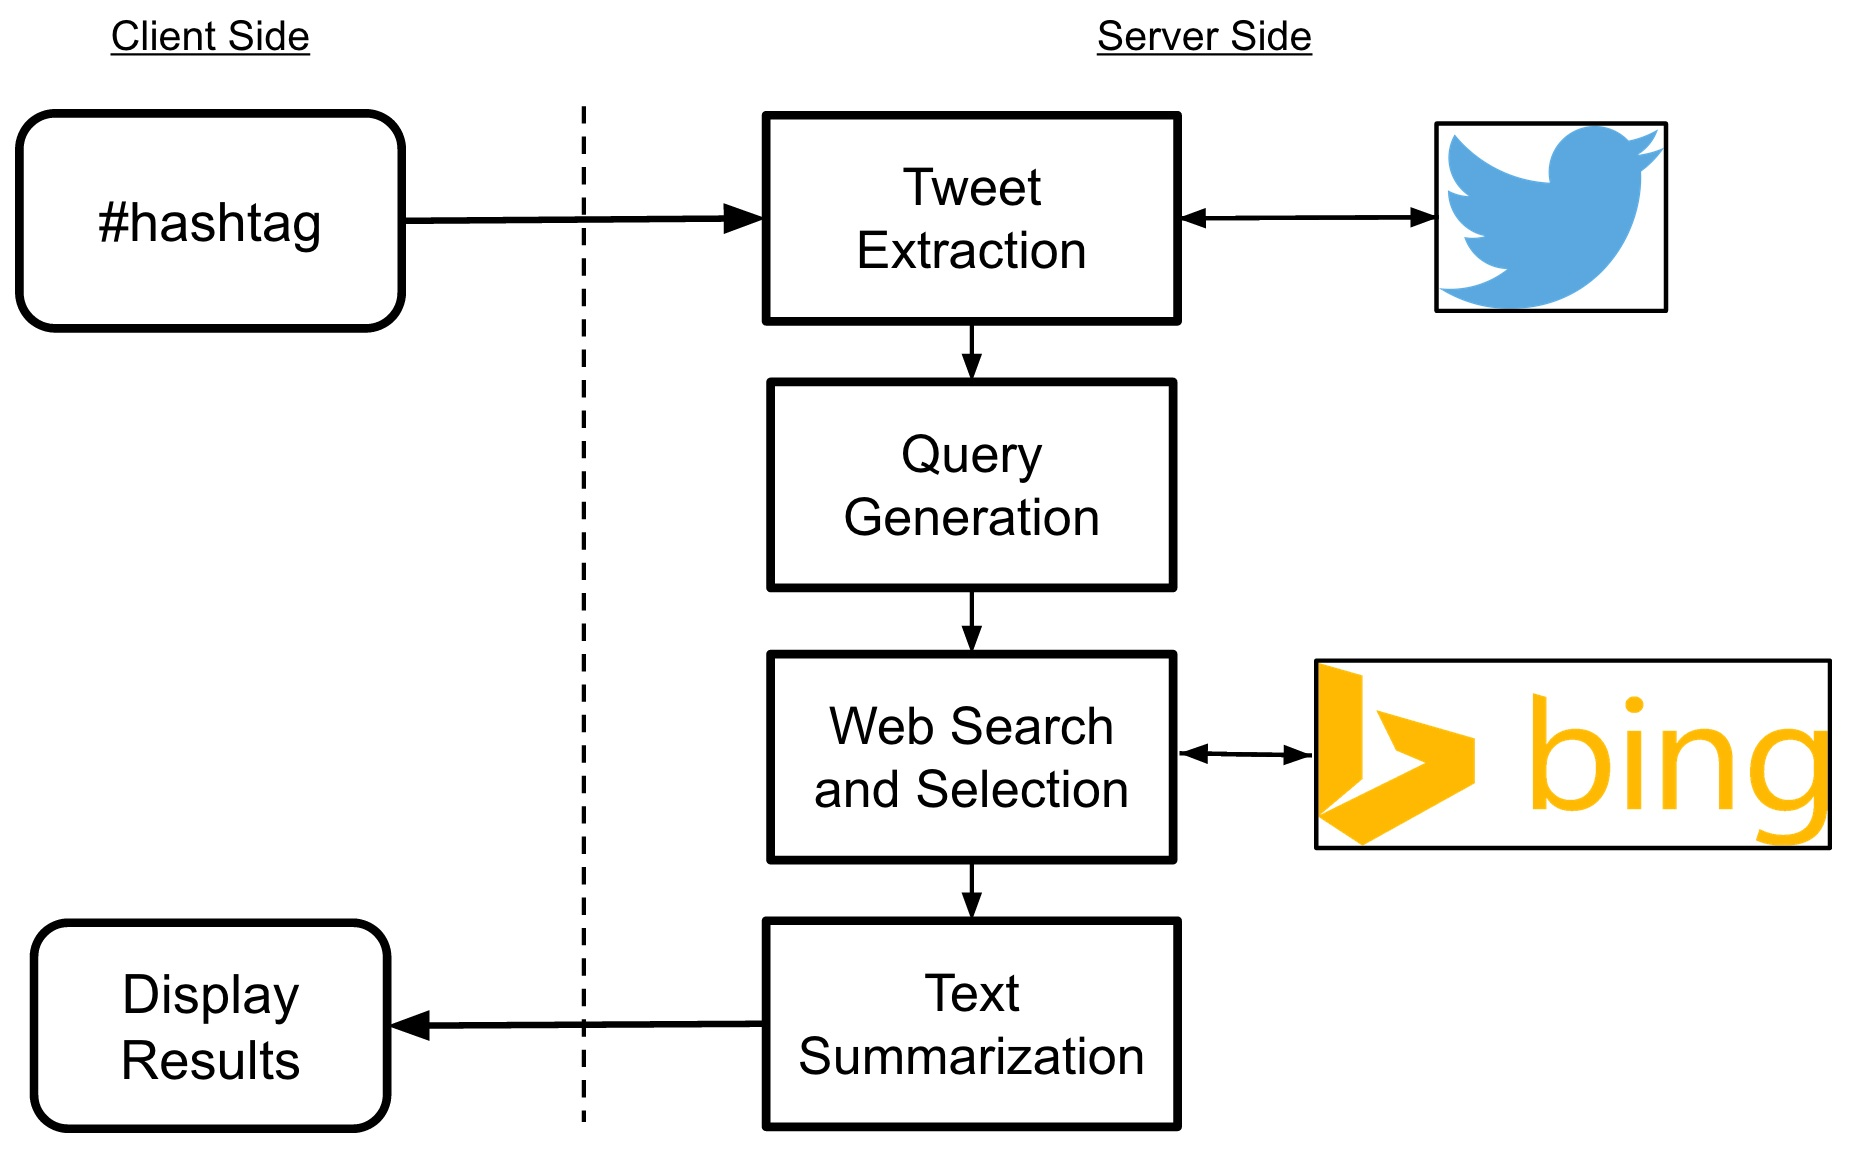
\includegraphics[width=.46\textwidth]{SystemArchitechture}}
   \caption{System Architechture} \label{fig:SystemArchitechture}
\end{figure}


\subsection{Tweet Extraction}
The Tweet Extraction module returns the text of the N most recent tweets that use the inquired hashtag using the Twitter Search API (we use N = 500 in our case). One limitation of this method is that currently, the Twitter Search API  only allows tweets from past 6-9 days. This makes it difficult to extract the meaning of hashtags that may have been used a few times in the past few days, but the majority of the times it was used was more than 6-9 days ago. \\
An important aspect of the tweet extraction is filtering the tweets that the search API retrieves. Firstly, we search the API using a '-filter:retweets' extension so that retweets are not considered because the top N most recent tweets very well may be all retweets. Secondly, we remove all URLS and emoticons from the tweets. We filter these out because emoticons cannot be used in a search engine search, and we make the assumption that the URLS that are included in tweets can be directly clicked on if they are relevant, so adding them to the query will not provide any additional relevant documents. In addition, we attempt to filter spam tweets by not including the text of tweets that have more than two trending hashtags. We understand that certain trending hashtags are sometimes correlated and thus are rightfully used together in a tweet, but we observed that most of the time spammers will use many trending hashtags in their tweets so that their tweets are seen by more viewers.
Since the Twitter search API is case-insensitive, we decide to manually filter out tweets that do not have the same case-sensitive hashtag. This is important because the case of certain letters can make a big difference of the hashtag meaning. For example, \#IAD refers to the Washington/Dulles international airport, but \#iAd refers to Apple's advertising platform). \\
Finally, we implement a "retrieve related hashtags" submodule which retrieves the top 5 most common co-occurring hashtags with the original inquired hashtag. This is useful due to the fact that often times the most common co-occurring hashtags are often related to the inquired hashtag, and may give more information about the inquired hashtag than it alone. This is a trivial task, but the user cannot parse all of the N most recent tweets and find the most common co-occurring hashtags, so it proves useful to be implemented in the plugin. The results of the tweet extraction module are then fed to the query generation module to be processed.

\subsection{Query Generation}
The main idea of the query generation module is to generate a query to search in Bing based on the text from the tweet extraction module. Our method generates a query based on the high-frequent terms from the tweets.\\
We first pre-process the filtered tweet text by using tokenization, case normalization, removing stopwords (which we added certain "twitter-specific" stopwords to the english stopwords list) and punctuation removal. We do not use stemming because we found that this in some cases resulted in a loss of information from the tweets, and a decreased accuracy. We also do not use segmentation because we found out that segmentation did not improve our results, and in some cases decreased accuracy. We assume that this is due to the fact that when we search something in Bing that contains concatenated words (e.g. 'presidentobama'), Bing does a better job segmenting the two words 'president' and 'obama' than the word segment toolkit. \\
We then counted the frequency of unigrams, bigrams, and trigrams that occur in the tweets. Based on this counting, we respectively sorted the uni-/bi-/tri-grams in descending order,  then created separate queries consisting of the following:
\begin{itemize}
	\item \{1st unigram\} (\textit{i.e.} Hashtag itself)
	\item \{1st unigram, 2nd unigram\}
	\item \{1st unigram, 2nd unigram, 3rd unigram\}
	\item \{2nd unigram, 3rd unigram\}
	\item \{1st bigram\}, if the frequency is above a certain threshold
	\item \{1st trigram\}, if the frequency is above a certain threshold
\end{itemize}

For example, the hashtag
\#Saban14, results in the following query vector: \\  
\big[ \{saban14\}, \{saban14 iran\}, \{saban14 iran clinton\},  \{iran clinton\}, \{saban forum\}, \{hillary clinton israel\} \big]\\
These queries do not explicitly tell you what \#Saban14 means, but when we search them on Bing.com, it gives good search results that are descriptive of the Saban 2014 Forum in the Middle East that is currently going on.

\subsection{Web Search and Selection}
Once the queries are generated, the next module performs separate searches on each of the generated queries using the Bing search API.  We take the top 2 search results from each of four subject domains over all queries: general web, bing news, wikipedia, and urban dictionary.  These different domains are intended to service different kinds of hashtags and information needs.  For instance, \#Saban2014 refers to a current event that should show up in news results.  \#WTS stands for Want To Sell, which is a common acronym/slang that UrbanDictionary explains. \#twitterblades refers to the fans of Sheffield United, a UK football team, and our system retrieves their Wikipedia page among the top links. \\
After getting results for all queries from each domain search, we apply a simple ranking strategy to order the urls in a reasonable manner.  URLs are weighted proportionately to the number of times they appear in search results of the various queries to various domains.  URLs are also weighted inversly to their position in per query rankings.  The product of these weights is taken to determine the merged result ranking.  The top 2 results from each subject domain are returned to the user.\\

\subsection{Text Summarization}
The final stage of the pipeline, before results are returned to the user, is document extraction and summarization.  Both are provided primarily by a publicly available Python library 'sumy.'  Extraction is performed with shall html parsing, while summaruzation is done with the LexRank.\cite{lexrank}  We choose LexRank for its purported ability to summarize the salient points of a noisy document cluster.  Unfortunately, this property either does not really exist, as it was not demonstrated in LexRank's initial evaluation, or cannot overcome the noise in the data provided to it.\\
The most obvious source of noises is hetergenous, and potentially irrelevant search results.  Given the variety and quality differentials of the various queries, we do not expect to always have the most relevant documents. Another source of noise is the shallow html parser that this library employs.  Unfortunately, many of the parsed sentences are simply related to the structure of parsed web pages and their operations.  Take, for example, this early attempt at create a summary for \#twitterblades: ``Retrieved 14 July 2013. Retrieved 9 July 2013. Retrieved 14 July 2013.''  All of these sentences are useless for summarization, but are highly related given their prevalence across different documents and within documents.  One heuristic to deal with such noise it require sentences contain at least 9 words.  Another possible solution to this problem is to rerank summary sentences with significant words from tweets, but this is not implemented in our system.

\section{Evaluation}
 At this time, we are not aware of any available "gold standard" dataset for hashtag meanings.  In order to compensate, we were forced to create our own test dataset, which consisted of a spreadsheet with 27 hashtags, and known relevant links to each of those hashtags. We understand that this is a small dataset, and not statistically significant, thus is a weak point of our system. Figure \ref{fig:recallat8} shows the results we got for the recall at 8 of the known relevant links that we annotated. We compare our model against a baseline methodology which looks at the top 8 retrieved results when searching the hashtag itself directly on Bing.com. 
\\There are a few takeaways from the results that we say. One important hashtag that our system performs worse in is \#Yosemite, which we annotated links to documents about Apple's newest operating system "Yosemite", but since we tested our evaluated weeks after Yosemite was released, many people were not talking about Apple's OS anymore, and were instead talking about Yosemite National park. Thus, our system returned documents related to the National Park, not the OS. In this way, it is important to note that our system is highly time-dependent for certain hashtags. One of the important properties of hashtags is that their meaning can vary depending on when they are used. In the same regard, our system can perform much better than our baseline method because of the temporal aspect in our system. For example, the hashtag \#LetsGoVCU refers to the Virginia Commonwealth basketball team, who recently made headlines for their game results, and thus there was much talk about them on Twitter using this hashtag. Since LetsGoVCU, is not a common search query, it did not perform well in our baseline. Table \ref{table:recall} shows the average recall at 8 results we achieved.
 
 \begin{figure}[h!]
     \fbox{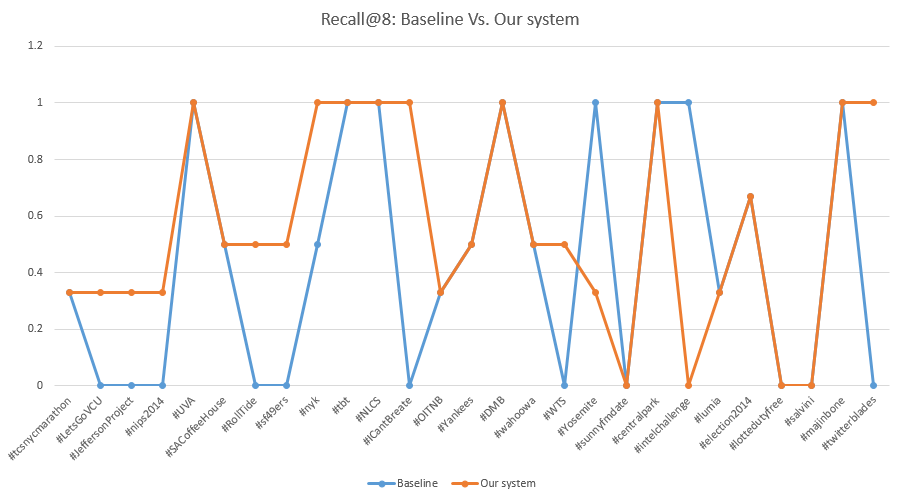
\includegraphics[width=.46\textwidth]{recallat8}}
   \caption{Evaluation results} \label{fig:recallat8}
\end{figure}



\begin{table}[h]
    \centering
    \caption[Table caption text]{Average recall@8.}
    \label{table:recall}
    \begin{tabular}{ | l | l | l |} \hline
    & Baseline & Our system \\ \hline
    Ave. recall@8 & 0.43 & 0.55 \\ \hline
    Matched Hashtags & 16/27 & 23/27 \\ \hline
    \end{tabular}
\end{table}
We did, in addition, do many heuristic based tests to see if we were getting relevant results based on the links that the system returned. We observed that in addition to noisy results, the system did often return at least one or two of the most relevant documents to a particular hashtag. The text summarization aspect did not perform very well, and we attribute this to the fact that in order to generate an accurate summary, the top few links returned must be very relevant to the hashtag, otherwise it will be a completely inaccurate summary.\\
\label{sec:evaluation}

\section{Conclusions and Future Work}
\label{sec:conclusions}
The main contribution of our work is a novel method of automatically extracting meaning from hashtags so that users can understand topics and trends more easily on Twitter. 
One aspect we wish to have implemented if we had more time was allowing the user to search for a hashtag from a certain tweet, and incorporating the text from that tweet (if efficient amount of text) more heavily than all of the others into the query generation. For example, if someone inquired about the hashtag \#UVA, our system would be able to return links with information about the University of Virginia. However, if the user was curious about the hashtag \#UVA in the context of a tweet that said something along the lines of 'The cavaliers remain undefeated in basketball this season', then the system should be able to extract words such as 'cavaliers' and 'basketball' in addition to 'UVA', and return links that relate to the University of Virginia basketball team. 

Evaluate based on the exact query generated terms.

%\subsection{References}
\bibliographystyle{acm}
\bibliography{sigproc}

\end{document}
